% Source: graduate-coursework/Research/Papers/drafts/autonomous_dataset_generation/Autonomous_Maritime_Radar_Dataset_Generation.tex
% Description: Camera-level YOLOv8-L verification loop: thermal and RGB frames (30 Hz) are independently processed by YOLOv8-L, confidence scores are averaged, and compared against threshold (0.7). If verified, frames and metadata are saved. If unverified but within 30-second timeout, RGB optical zoom increases by 5x increments and inference repeats. After timeout, detection is marked false alarm and system advances to next queued target.

\documentclass[border=4pt]{standalone}
\usepackage{algpseudocode}
\usepackage{amsmath, amssymb}
\usepackage{graphicx}
\usepackage{tikz}

\newcommand{\PlaceHolder}[2]{%
  \fbox{%
    \begin{minipage}[c][#2][c]{#1}
      \centering\small
      FIGURE PLACEHOLDER\\
      Replace with final artwork
    \end{minipage}%
  }%
}

\begin{document}
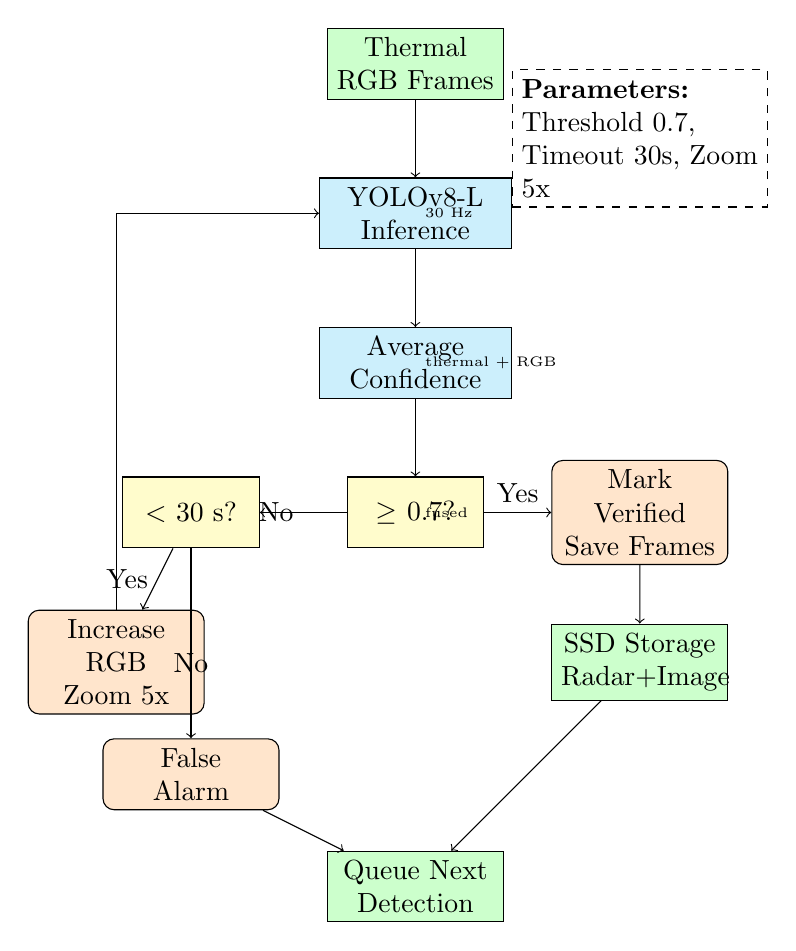
\begin{tikzpicture}[node distance=2cm, auto, scale=0.95]
  % Define styles
  \tikzstyle{process} = [rectangle, draw, fill=cyan!20, text width=2.2cm, text centered, minimum height=0.7cm]
  \tikzstyle{decision} = [rectangle, draw, fill=yellow!20, text width=1.5cm, text centered, minimum height=0.9cm]
  \tikzstyle{action} = [rectangle, draw, fill=orange!20, text width=2cm, text centered, rounded corners, minimum height=0.7cm]
  \tikzstyle{io} = [rectangle, draw, fill=green!20, text width=2cm, text centered, minimum height=0.7cm]

  % Start
  \node[io] (start) at (0,5.5) {Thermal\\RGB Frames};

  % YOLOv8 inference
  \node[process] (yolo) at (0,3.5) {YOLOv8-L\\Inference};

  % Confidence fusion
  \node[process] (fuse) at (0,1.5) {Average\\Confidence};

  % Decision
  \node[decision] (conf) at (0,-0.5) {$\geq 0.7$?};

  % Yes path - verified
  \node[action] (verify) at (3,-0.5) {Mark Verified\\Save Frames};

  % No path - check timeout
  \node[decision] (timeout) at (-3,-0.5) {$< 30$ s?};

  % Zoom increase
  \node[action] (zoom) at (-4,-2.5) {Increase RGB\\Zoom 5x};

  % False alarm
  \node[action] (alarm) at (-3,-4) {False\\Alarm};

  % Next target
  \node[io] (next) at (0,-5.5) {Queue Next\\Detection};

  % Storage
  \node[io] (storage) at (3,-2.5) {SSD Storage\\Radar+Image};

  % Connections - main flow
  \draw[->] (start) -- (yolo) node[right, font=\tiny] {30 Hz};
  \draw[->] (yolo) -- (fuse) node[right, font=\tiny] {thermal + RGB};
  \draw[->] (fuse) -- (conf) node[right, font=\tiny] {fused};

  % Verified path (Yes)
  \draw[->] (conf) -- node[above] {Yes} (verify);
  \draw[->] (verify) -- (storage);
  \draw[->] (storage) -- (next);

  % Unverified path (No)
  \draw[->] (conf) -- node[left] {No} (timeout);

  % Timeout decision
  \draw[->] (timeout) -- node[left] {Yes} (zoom);
  \draw[->] (zoom) |- (yolo);
  \draw[->] (timeout) -- node[below] {No} (alarm);
  \draw[->] (alarm) -- (next);

  % Add parameter box
  \node[rectangle, draw, dashed, fill=white, text width=3cm] at (3,4.5) {\textbf{Parameters:} Threshold 0.7, Timeout 30s, Zoom 5x};

\end{tikzpicture}
\end{document}
